% Figure from MATH 591 notes, section 33. Compile with the notes preamble.
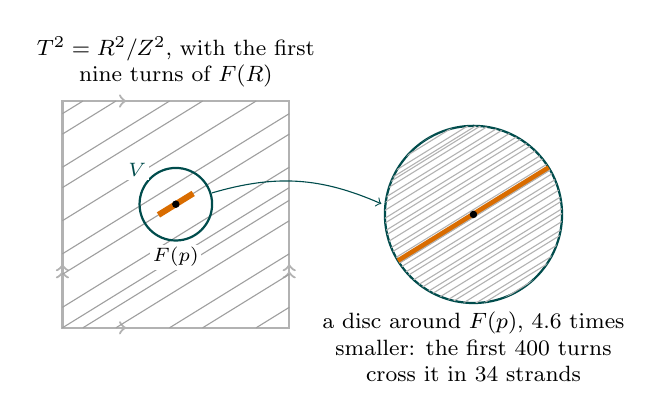
\begin{tikzpicture}[scale=0.9]
\draw[gray!60, thick] (0,0) rectangle (3.20,3.20);
\draw[->, gray!60, thick] (0.5,0) -- (0.9,0); \draw[->, gray!60, thick] (0.5,3.20) -- (0.9,3.20); \draw[->>, gray!60, thick] (0,0.5) -- (0,0.9); \draw[->>, gray!60, thick] (3.20,0.5) -- (3.20,0.9);
\draw[gray!75] (0.000,0.000) -- (3.200,1.978);
\draw[gray!75] (0.000,1.978) -- (1.978,3.200);
\draw[gray!75] (1.978,0.000) -- (3.200,0.755);
\draw[gray!75] (0.000,0.755) -- (3.200,2.733);
\draw[gray!75] (0.000,2.733) -- (0.755,3.200);
\draw[gray!75] (0.755,0.000) -- (3.200,1.511);
\draw[gray!75] (0.000,1.511) -- (2.733,3.200);
\draw[gray!75] (2.733,0.000) -- (3.200,0.289);
\draw[gray!75] (0.000,0.289) -- (3.200,2.266);
\draw[gray!75] (0.000,2.266) -- (1.511,3.200);
\draw[gray!75] (1.511,0.000) -- (3.200,1.044);
\draw[gray!75] (0.000,1.044) -- (3.200,3.022);
\draw[gray!75] (0.000,3.022) -- (0.289,3.200);
\draw[gray!75] (0.289,0.000) -- (3.200,1.799);
\draw[orange!85!black, line width=2.2pt] (1.355,1.593) -- (1.845,1.896);
\draw[teal!60!black, thick] (1.600,1.744) circle (0.512);
\fill (1.600,1.744) circle (1.5pt);
\node[font=\scriptsize, fill=white, inner sep=1pt, anchor=north] at (1.600,1.182) {$F(p)$};
\node[teal!60!black, font=\scriptsize, fill=white, inner sep=1pt] at (1.056,2.224) {$V$};
\node[font=\footnotesize, align=center] at (1.60,3.75) {$T^2 = \mathbb{R}^2/\mathbb{Z}^2$, with the first\\ nine turns of $F(\mathbb{R})$};
\draw[teal!60!black, thick] (5.80,1.60) circle (1.25);
\begin{scope}\clip (5.80,1.60) circle (1.25);
\draw[orange!85!black, line width=2pt] (4.439,0.759) -- (7.161,2.441);
\draw[gray!60] (3.889,1.649) -- (6.611,3.331);
\draw[gray!60] (4.779,0.209) -- (7.501,1.891);
\draw[gray!60] (4.229,1.099) -- (6.951,2.781);
\draw[gray!60] (4.569,0.549) -- (7.291,2.231);
\draw[gray!60] (4.019,1.439) -- (6.741,3.121);
\draw[gray!60] (4.909,-0.001) -- (7.631,1.681);
\draw[gray!60] (4.359,0.889) -- (7.081,2.571);
\draw[gray!60] (3.809,1.779) -- (6.531,3.461);
\draw[gray!60] (4.699,0.339) -- (7.421,2.021);
\draw[gray!60] (4.149,1.229) -- (6.871,2.911);
\draw[gray!60] (5.039,-0.212) -- (7.761,1.471);
\draw[gray!60] (4.489,0.679) -- (7.211,2.361);
\draw[gray!60] (3.938,1.569) -- (6.661,3.251);
\draw[gray!60] (4.829,0.128) -- (7.551,1.811);
\draw[gray!60] (4.278,1.019) -- (7.001,2.701);
\draw[gray!60] (4.618,0.468) -- (7.341,2.151);
\draw[gray!60] (4.068,1.359) -- (6.790,3.041);
\draw[gray!60] (4.958,-0.082) -- (7.680,1.601);
\draw[gray!60] (4.408,0.808) -- (7.130,2.491);
\draw[gray!60] (3.858,1.699) -- (6.580,3.381);
\draw[gray!60] (4.748,0.258) -- (7.470,1.941);
\draw[gray!60] (4.198,1.148) -- (6.920,2.831);
\draw[gray!60] (5.088,-0.292) -- (7.810,1.391);
\draw[gray!60] (4.538,0.598) -- (7.260,2.281);
\draw[gray!60] (3.988,1.488) -- (6.710,3.171);
\draw[gray!60] (4.878,0.048) -- (7.600,1.731);
\draw[gray!60] (4.328,0.938) -- (7.050,2.621);
\draw[gray!60] (3.778,1.828) -- (6.500,3.511);
\draw[gray!60] (4.668,0.388) -- (7.390,2.071);
\draw[gray!60] (4.118,1.278) -- (6.840,2.961);
\draw[gray!60] (5.008,-0.162) -- (7.730,1.520);
\draw[gray!60] (4.458,0.728) -- (7.180,2.411);
\draw[gray!60] (3.908,1.618) -- (6.630,3.301);
\end{scope}
\fill (5.80,1.60) circle (1.5pt);
\draw[->, teal!60!black] (2.112,1.904) to[bend left=20] (4.50,1.75);
\node[font=\footnotesize, align=center] at (5.80,-0.27) {a disc around $F(p)$, 4.6 times\\ smaller: the first 400 turns\\ cross it in 34 strands};
\end{tikzpicture}
